\documentclass{beamer}
\usepackage{beamerthemesplit} % new

\usepackage[utf8]{inputenc}

\begin{document}
\title{Perdidos en la ignorancia}
\author{ES\_2019\_G43-2-02}
\date{\today}

\frame{\titlepage}

\frame{\frametitle{Table of contents}\tableofcontents}


\section{Membres del equip}
\frame{\frametitle{Team}
  \begin{itemize}
    \item Aleksandra Jovanovic
    \item Daniel Montesinos Santos
    \item Adrián Moreno Gimeno
    \item Núria Navarro Juliana
    \item Desirée Pasión Rodriguez Sanchez
  \end{itemize}
}


\section{Jira}
\subsection{Product Backlog/Tasques}
\frame{\frametitle{Product Backlog}
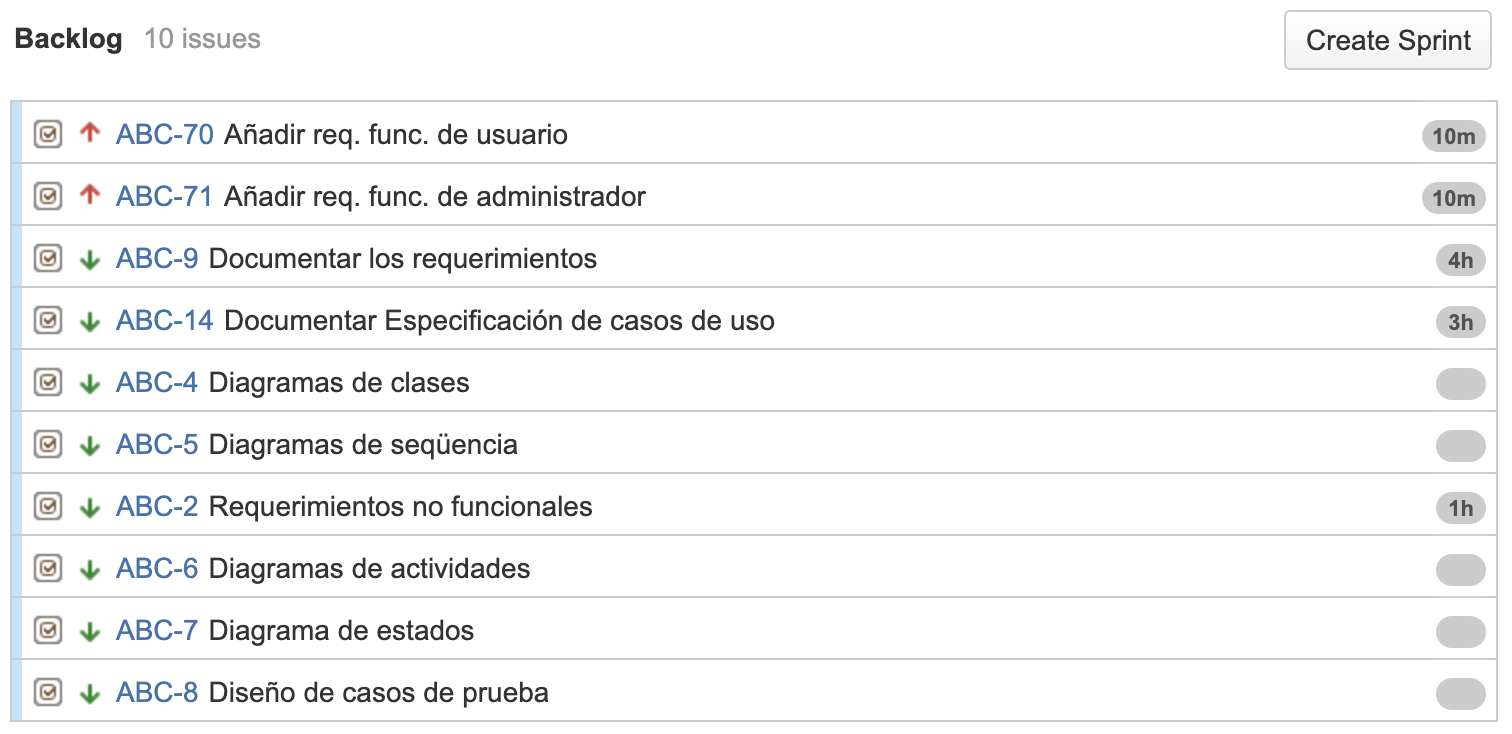
\includegraphics[width=1\textwidth]{./imatges/ProductBacklog2.png}
}

\frame{\frametitle{Tasques}
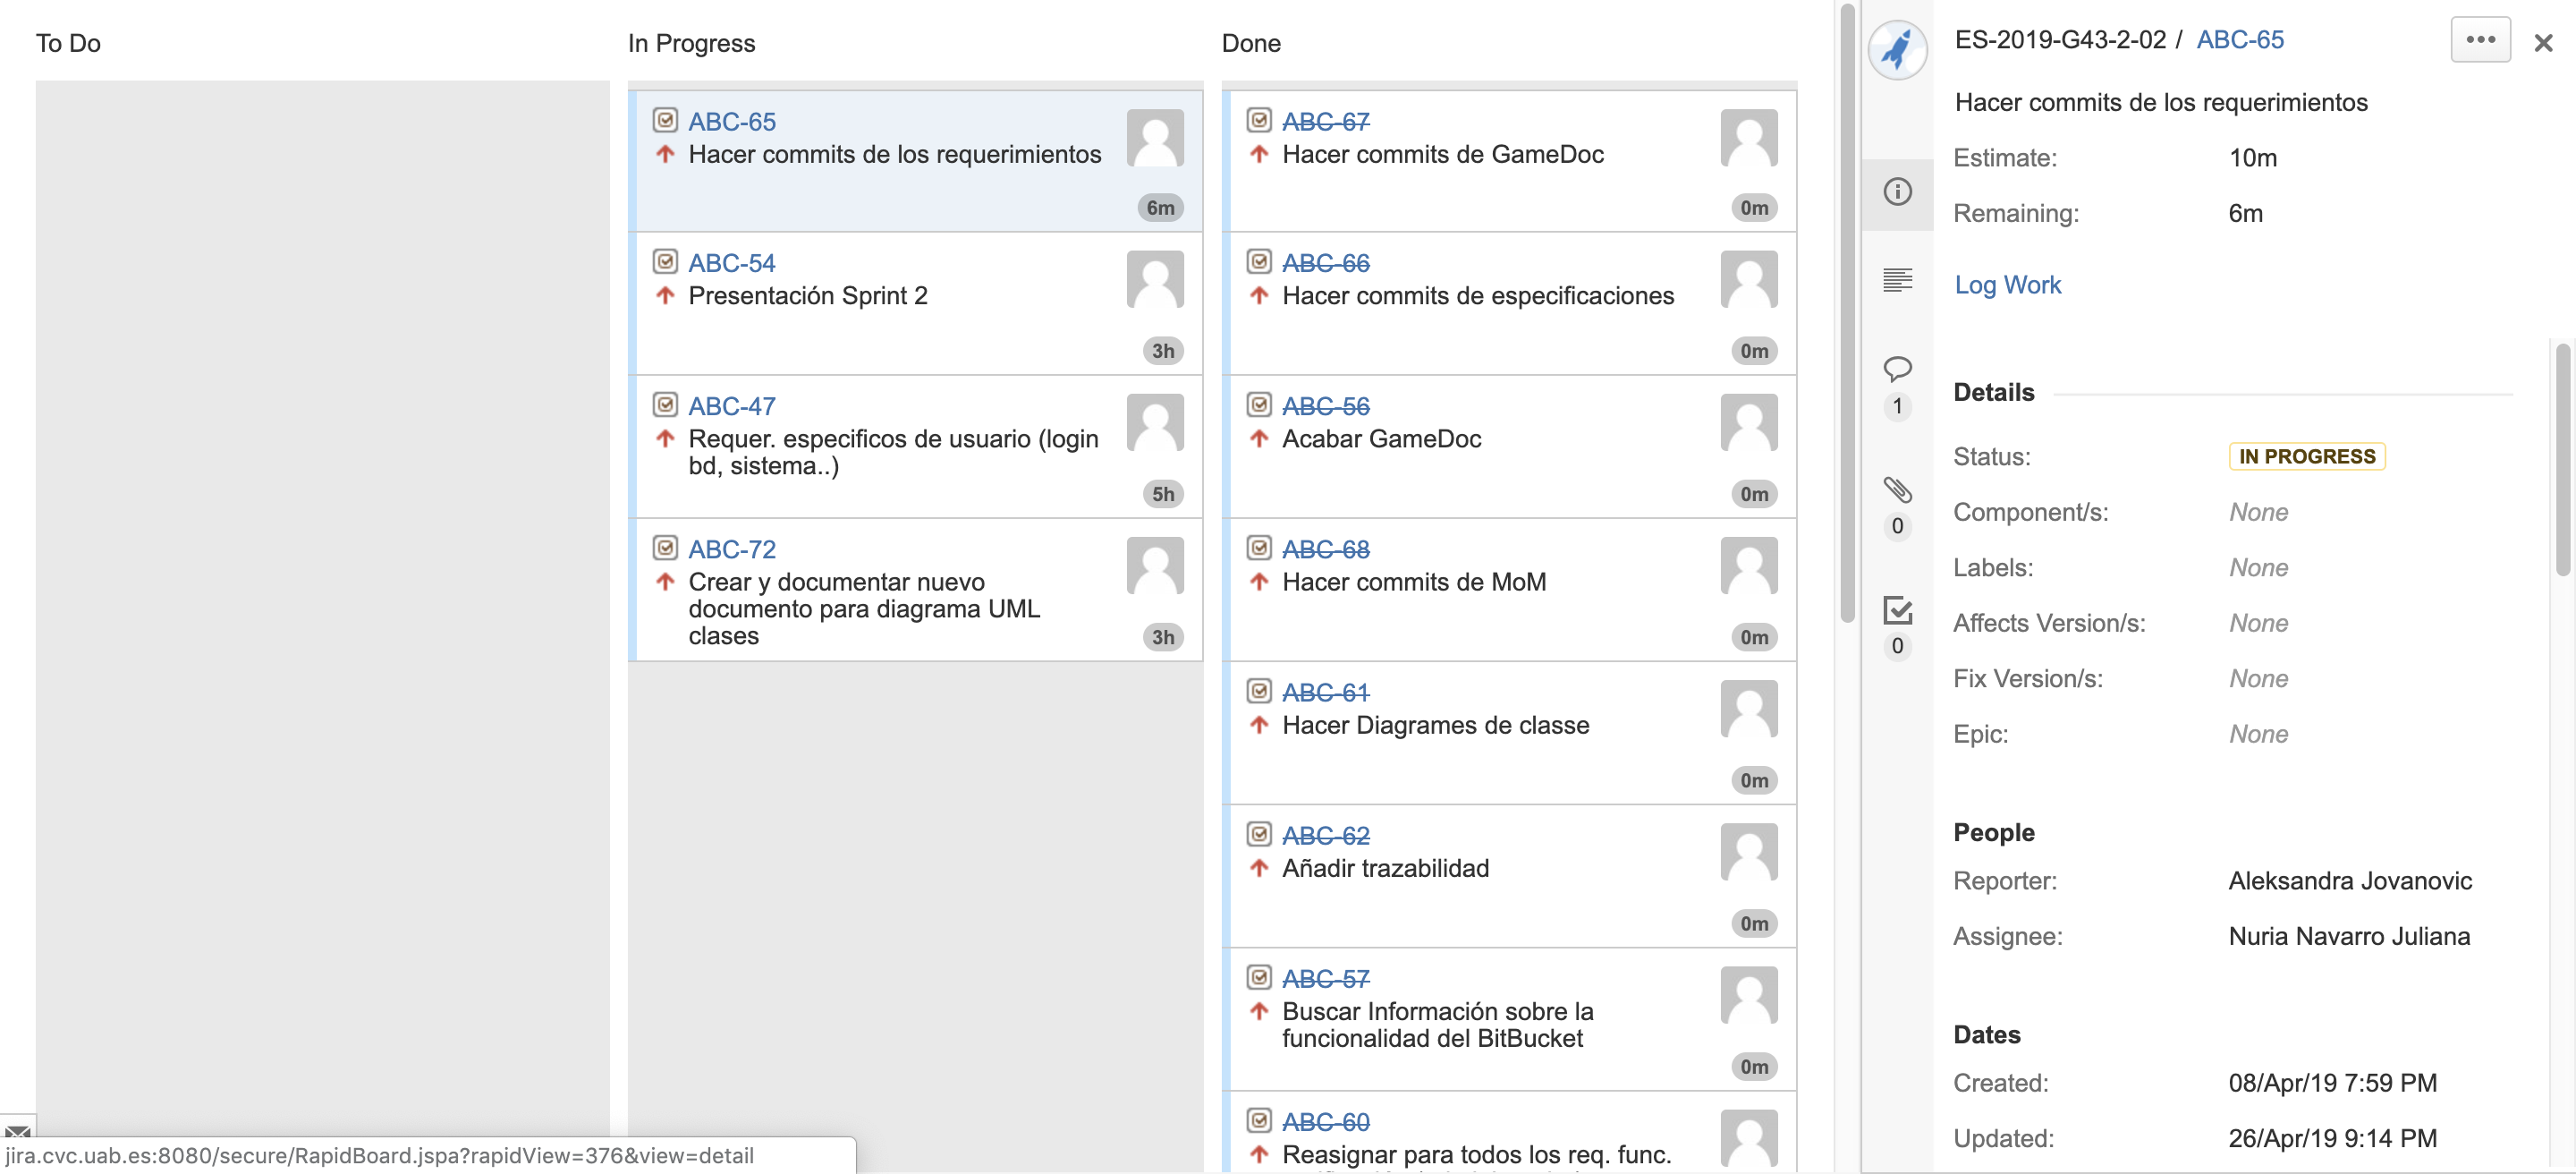
\includegraphics[width=1\textwidth]{./imatges/tareas2.png}
}

\subsection{Burndown chart}
\frame{\frametitle{Burndown chart}

  \begin{figure}[ht]
  \centering
  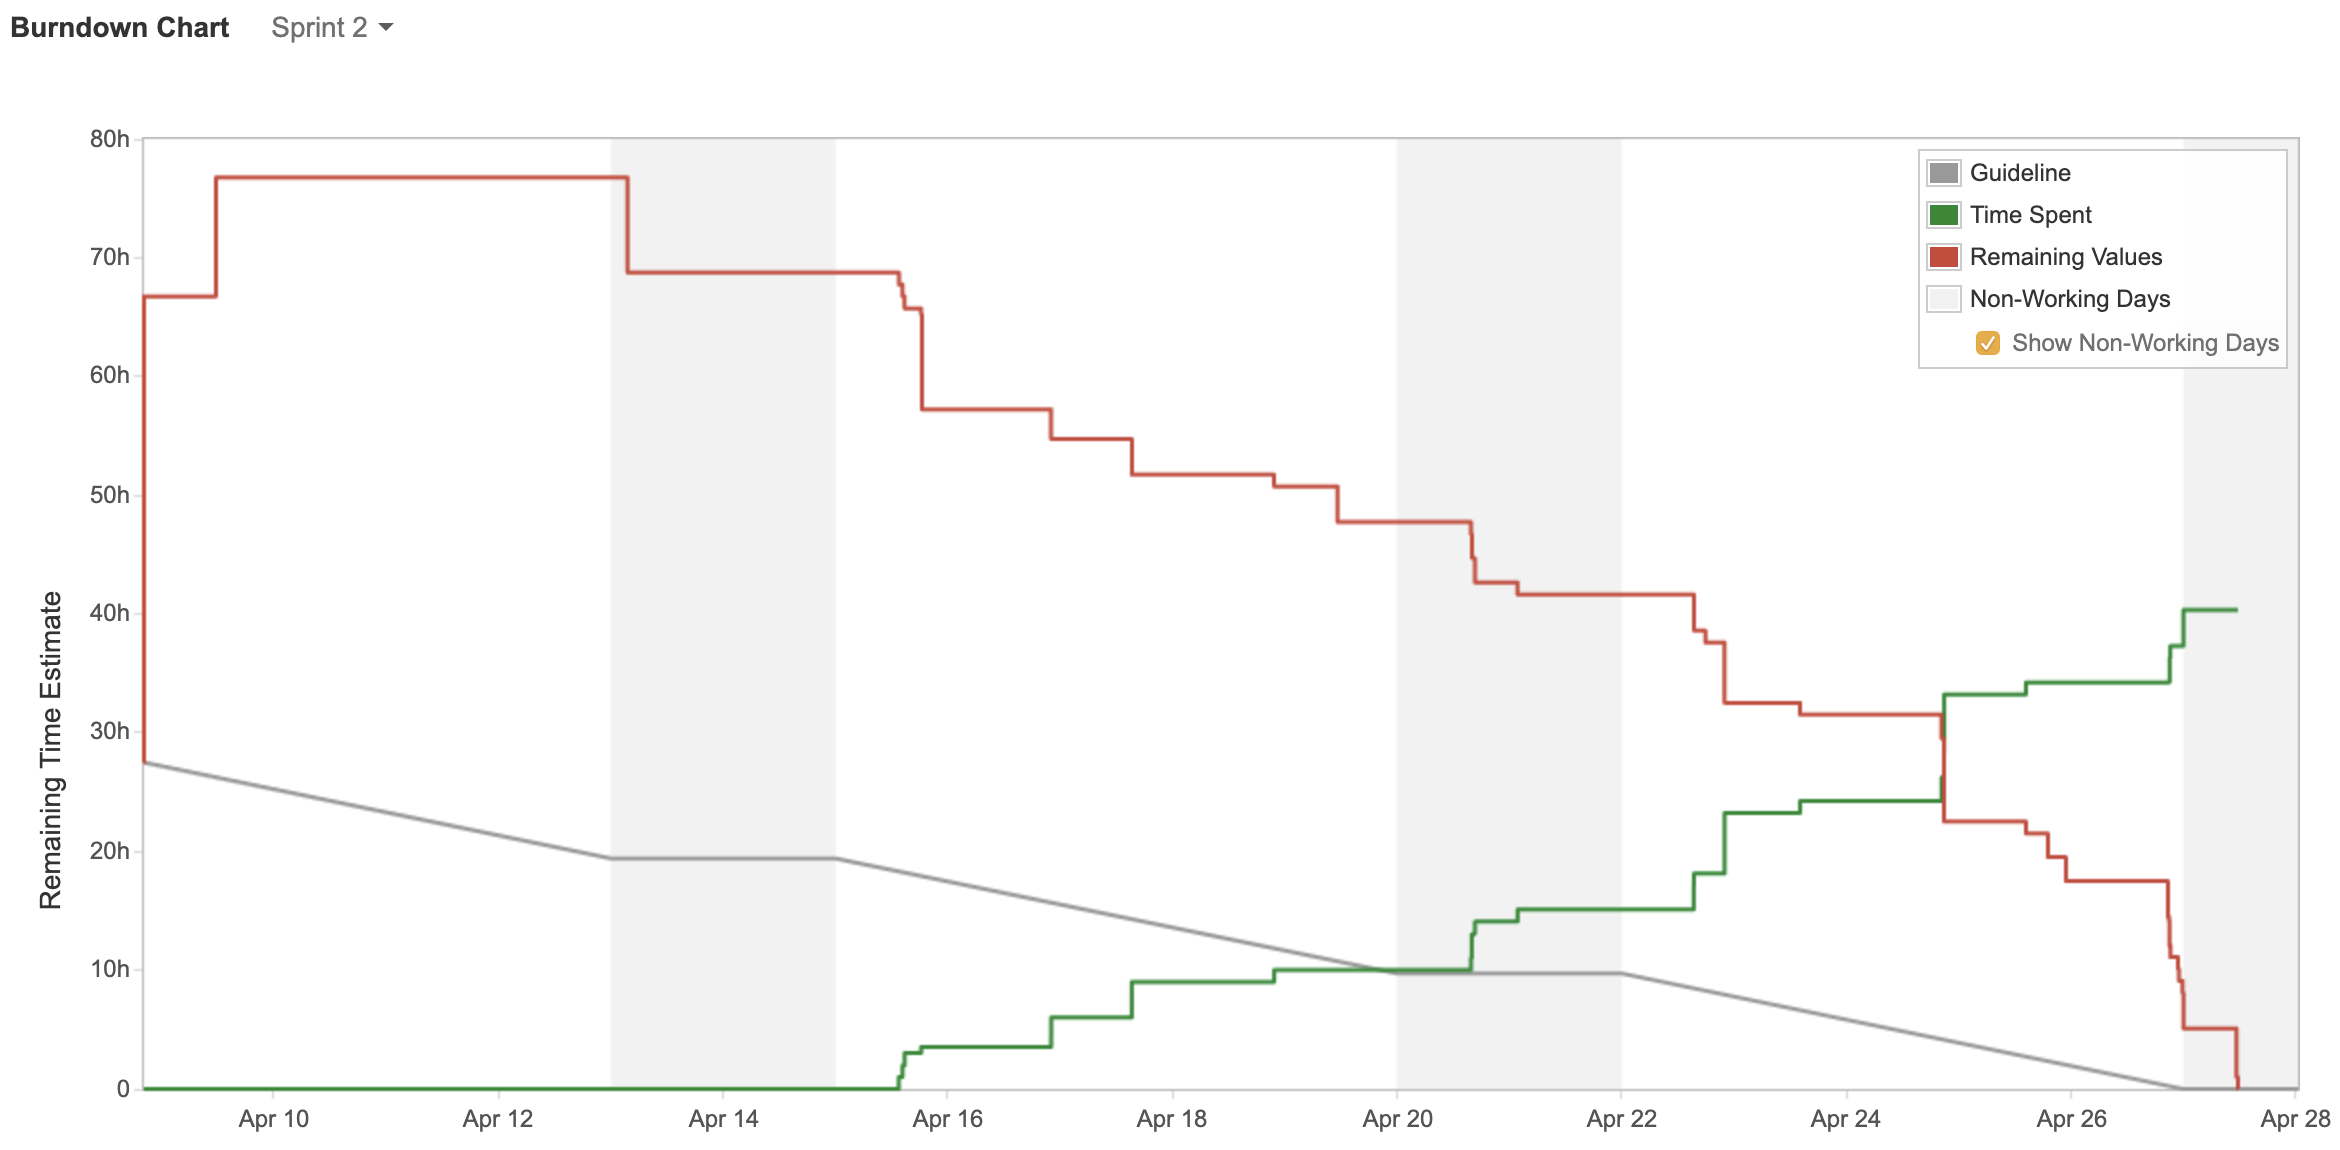
\includegraphics[width=1\textwidth]{./imatges/burndown2.png}
  \label{fig:bdchart}
\end{figure}

}

\section{Bitbucket}
\frame{\frametitle{Bitbucket}
\begin{center}
	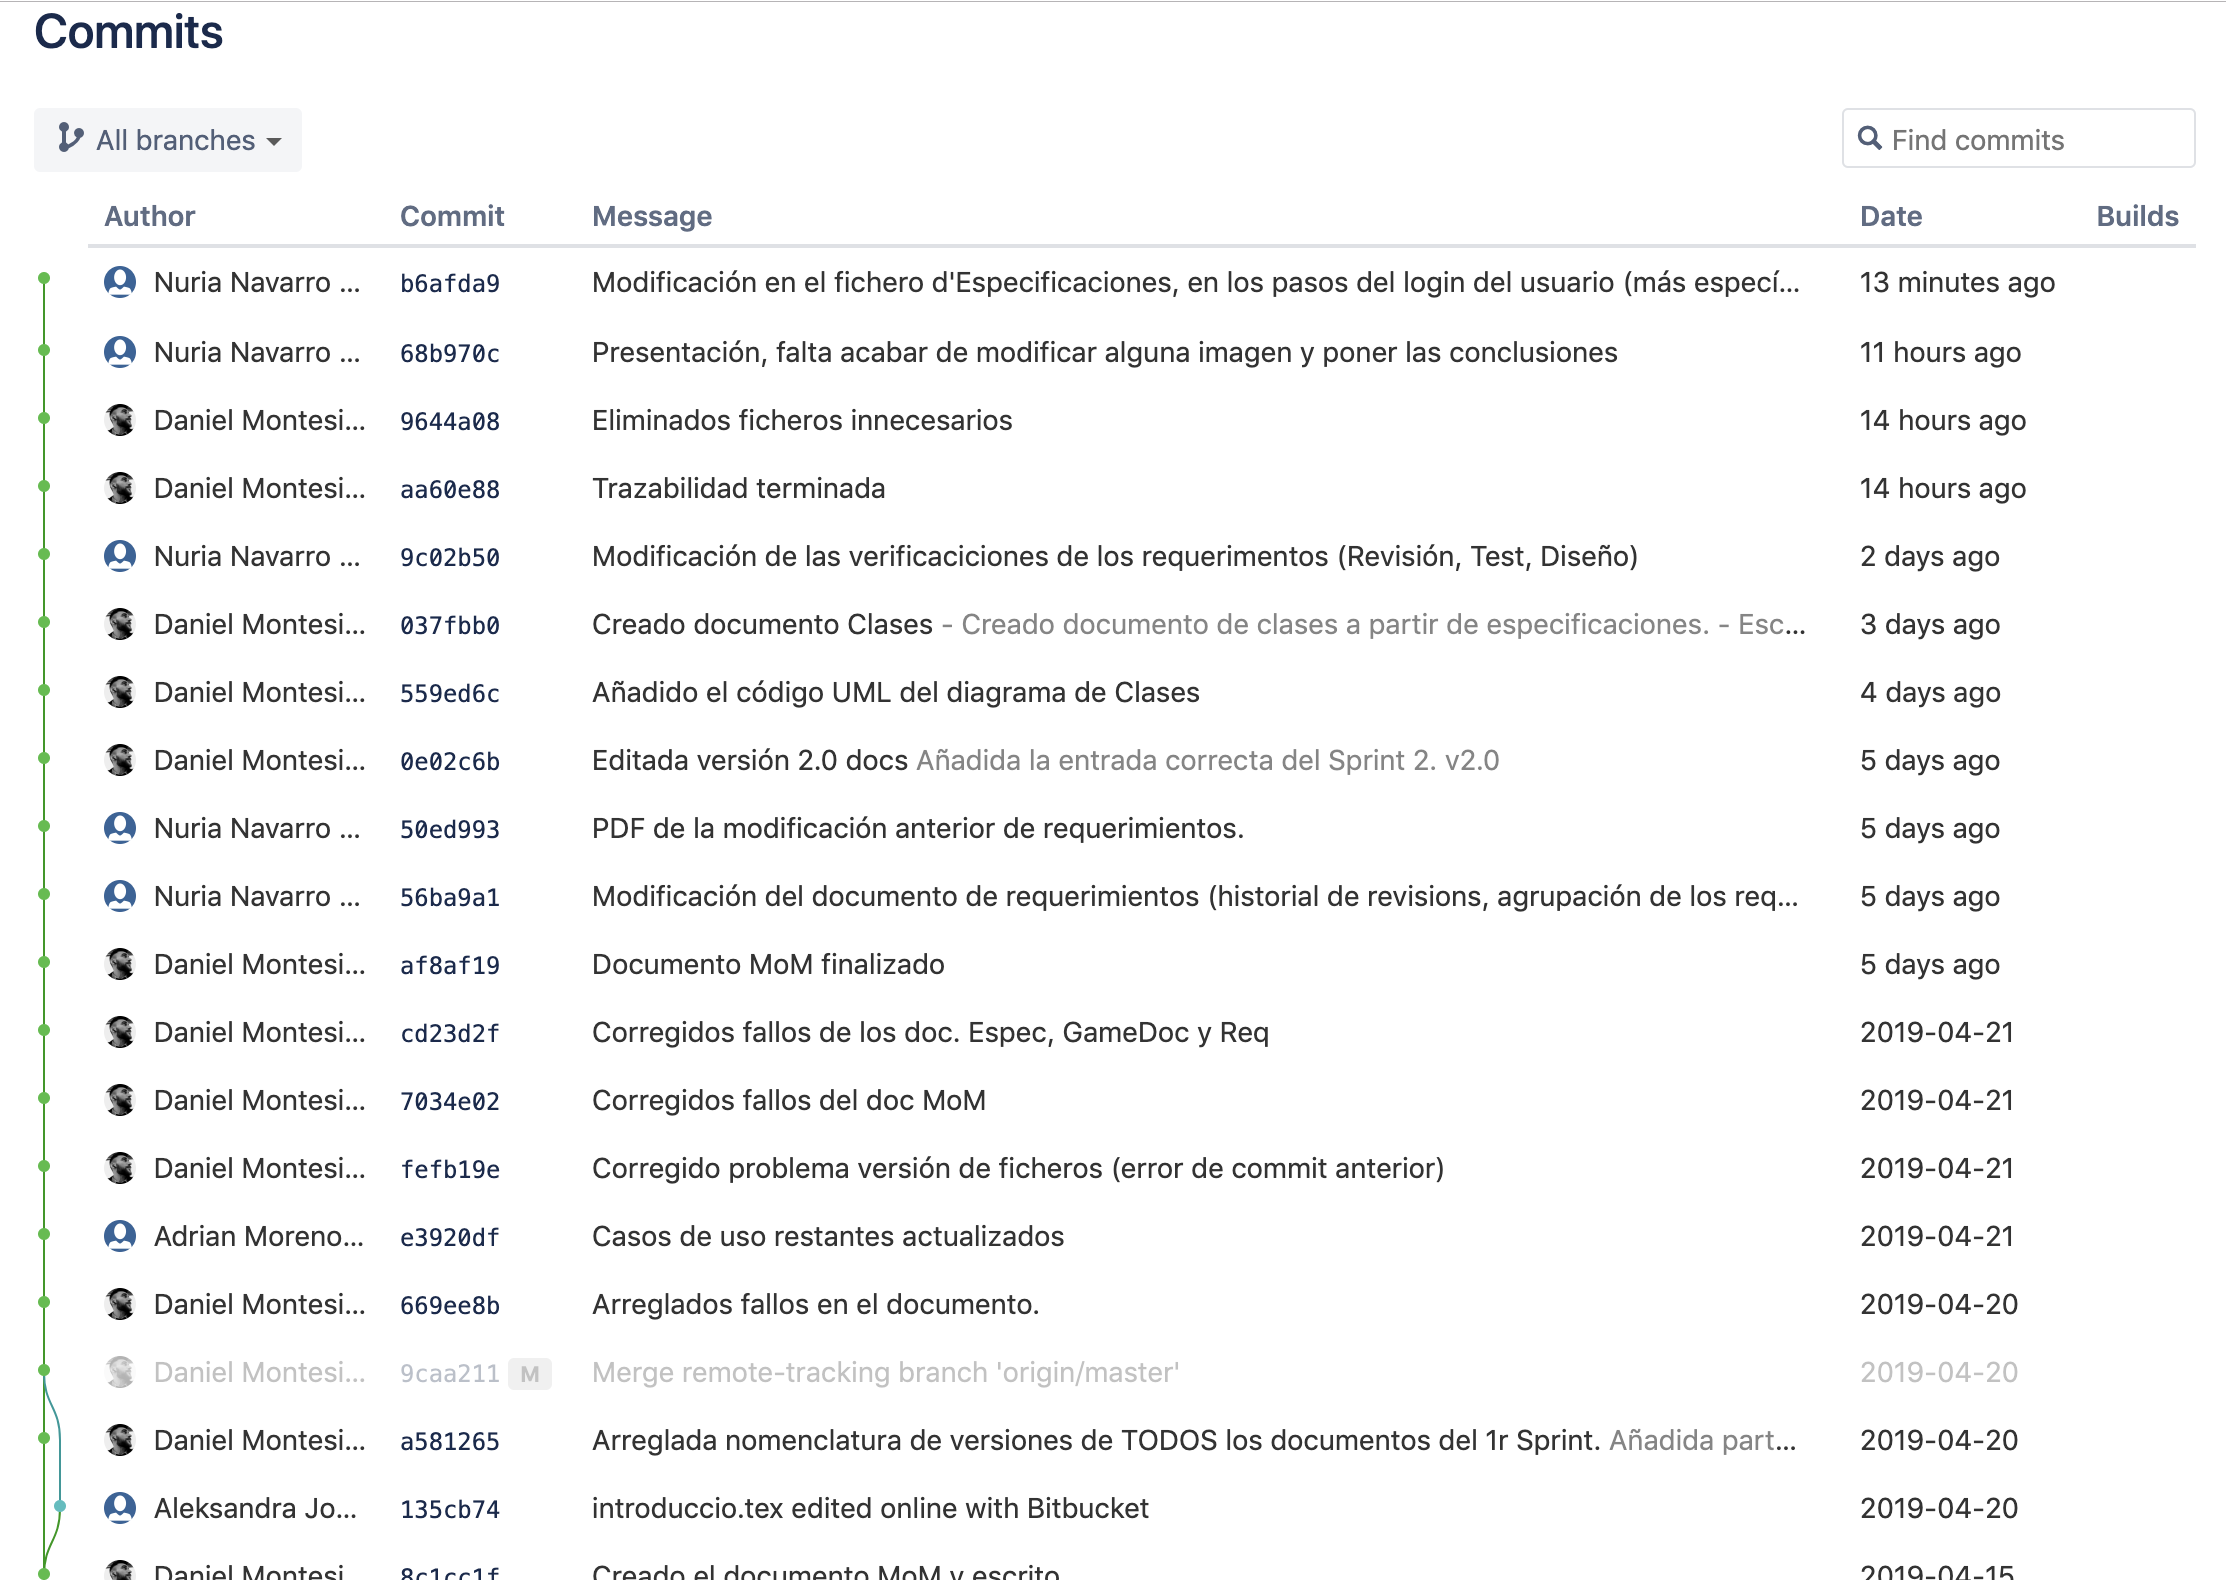
\includegraphics[width=0.8\textwidth]{./imatges/bitbucket2.png}
\end{center}
}


\section{Classes}
\frame{\frametitle{Classes}
\begin{center}
	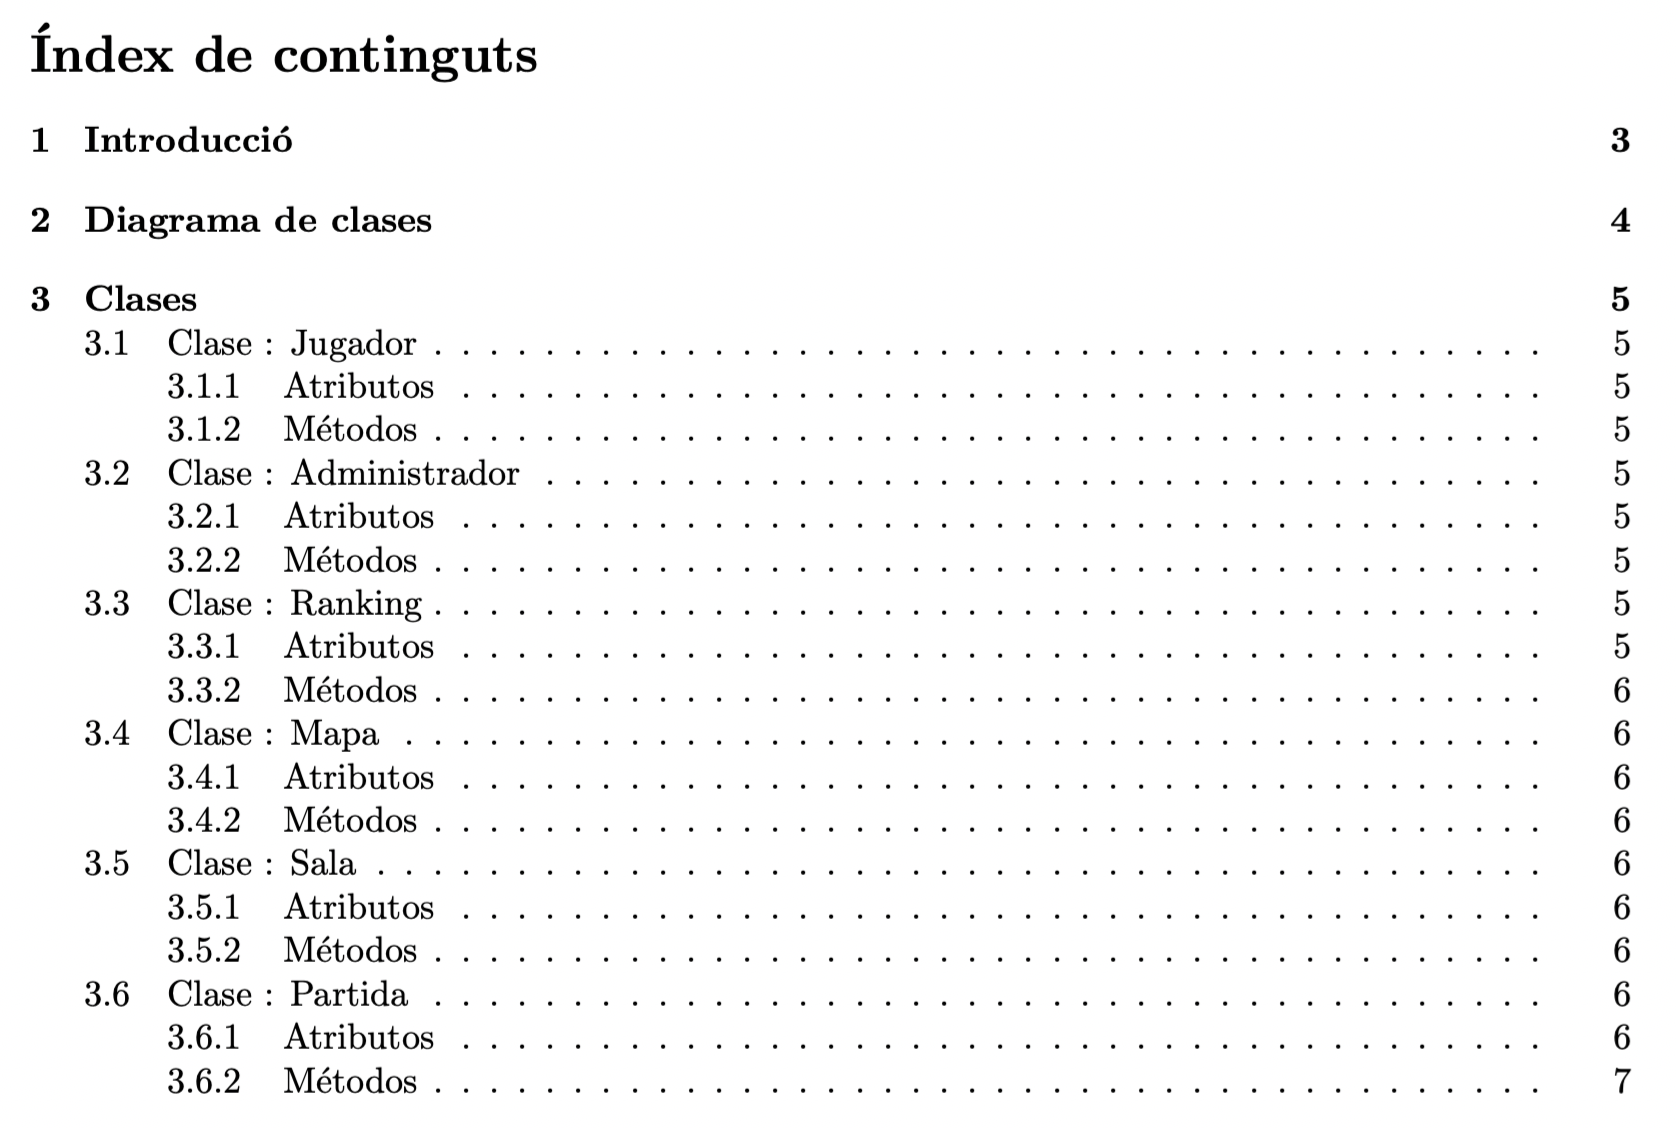
\includegraphics[width=0.8\textwidth]{./imatges/Clases.png}
\end{center}
}


\section{Diagrama de Classes}
\frame{\frametitle{Diagrama de Classes}
\begin{center}
	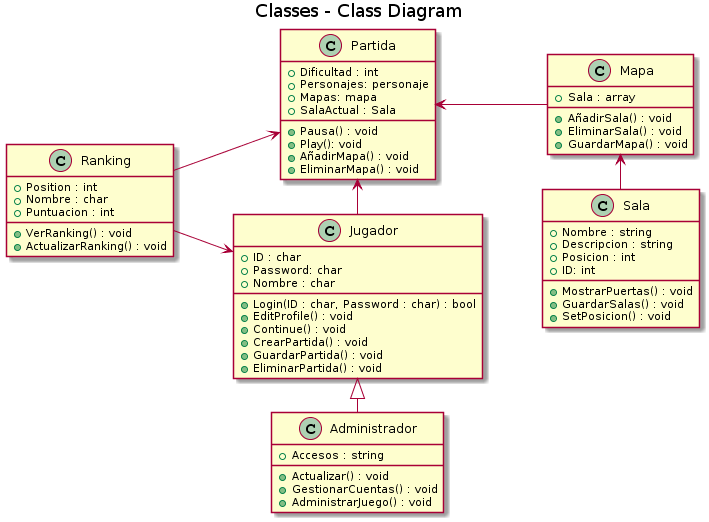
\includegraphics[width=0.8\textwidth]{./imatges/DiagramaClases.png}
\end{center}
}


\section{Conclusions}
\frame{\frametitle{Conclusions}
\begin{enumerate}
\item Hemos mejorado la intuición de la duración de las tareas.
\item Hemos modificado los errores del anterior sprint.
\item Mejor organización, trabajo progresivo.

\end{enumerate}
}

\end{document}
